\documentclass[10pt,aspectratio=169]{beamer}
\usepackage[utf8]{inputenc}

\usepackage{tikz}
\usepackage{multimedia}
\usepackage{hyperref}
\usepackage{graphicx,epsfig}
\graphicspath{{figure/}} 

\usetheme{Madrid}
\usecolortheme{default}
\setbeamertemplate{caption}[numbered]

\title[MCL-738]
{Dynamic Analysis of Four Bar Mechanism}

\author[IIT Delhi]
{Vinay Kumar\inst{1} \and Naveen Kumar Sahu\inst{1}}

\institute[]
{
  \inst{1}%
  Mechanical Department\\
  IIT Delhi
  \and

}

\date[\today]{MCL 738 : Multibody Dynamics}

\begin{document}	
\frame{\titlepage}

\section{Introduction}

\begin{frame}
\frametitle{The Long And Short of Analysis}
\begin{columns}
	\begin{column}{8cm}
	\begin{itemize}
		\item Formulated lagrangian based equation of motion for four bar mechanism
		\item Reduced all the expression to those of $\theta$
		\item Created a interactive geometric construction in Cinderella Geometry \cite{Cindy} for verifying Inverse Kinematics (Angles and Velocities)
		\item Computed inverse dynamics for \alert{\href{run:./figure/crankCrank1Inverse.avi}{cycloidal motion}} of input link
		\item Applied the computed torques to four bar mechanism for \alert{\href{run:./figure/crankCrank1Forward.avi}{forward dynamics}}
	\end{itemize}
	\end{column}
	\begin{column}{6cm}
		\centering
	\begin{figure}
		\centering
		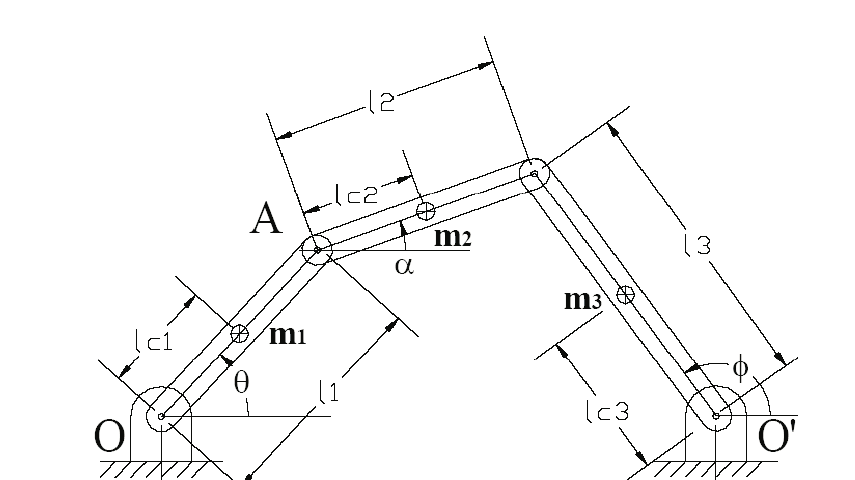
\includegraphics[width=6cm,keepaspectratio]{notation}
		\caption{Symbols used. Source:\cite{tang2006lagrangian}}
	\end{figure}
	\end{column}
\end{columns}
\end{frame}

\begin{frame}
\frametitle{Features of Code}
\begin{itemize}
	\item Can carry out analysis for all types of Grashof's mechanisms i.e. Crank-Crank, Crank-Rocker, Rocker-Crank and Rocker-Rocker
	\item Checks if the mechanism is \textit{possible} for the given link lengths
	\item Can take different modes of assembly (elbow-up, elbow-down) as input
	\item Computes the possible range of motion for mechanism
	\item Takes care of mechanical limits in case the mechanism have one or more rocker linkages
	\item Decides the type of four bar mechanism and exits accordingly for special cases \cite{wiki:fourBar}
\end{itemize}
\end{frame}

\begin{frame}
\frametitle{Heuristics for restarting ODE}
\begin{itemize}
	\item Based on event detection whenever the mechanism hits a mechanical limits, its velocity is reversed and reduced by 10\%
	\item However the ode sometimes still goes in region of in-feasible configurations, in such cases the error is caught by a try \& catch statement; and the ode is restarted with a reduced maximum time step and a slightly incremented starting time $0.1\; second$.
\end{itemize}

\begin{columns}
	\begin{column}{4cm}
	\begin{figure}
		\centering
		\href{run:./figure/rockerCrank1Forward.avi}{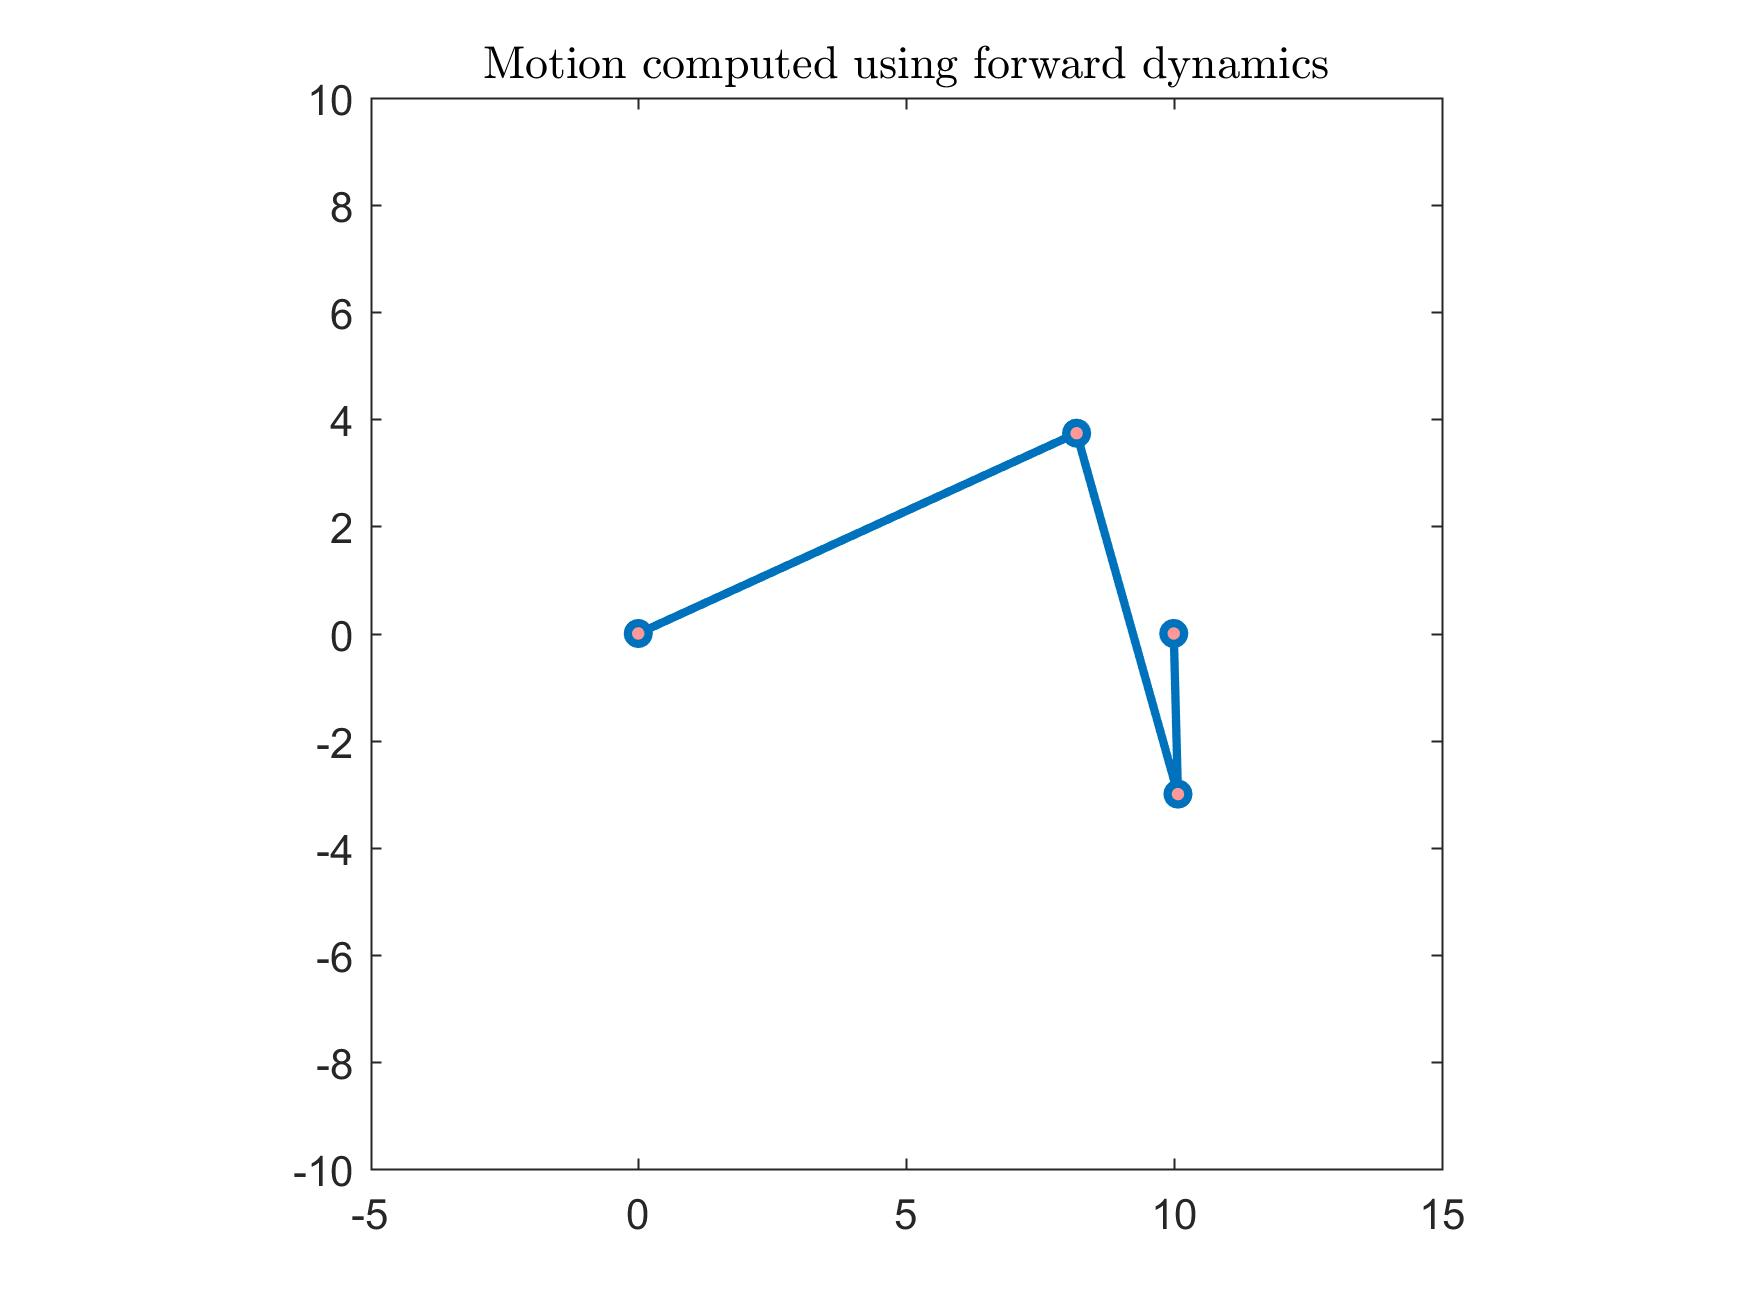
\includegraphics[width=4cm,keepaspectratio]{rockerCrank1banner}}
		\caption{\scriptsize{Rocker Crank One}}
	\end{figure}

	\end{column}
	\begin{column}{4cm}
		\begin{figure}
		\centering
		\href{run:./figure/rockerCrank2Forward.avi}{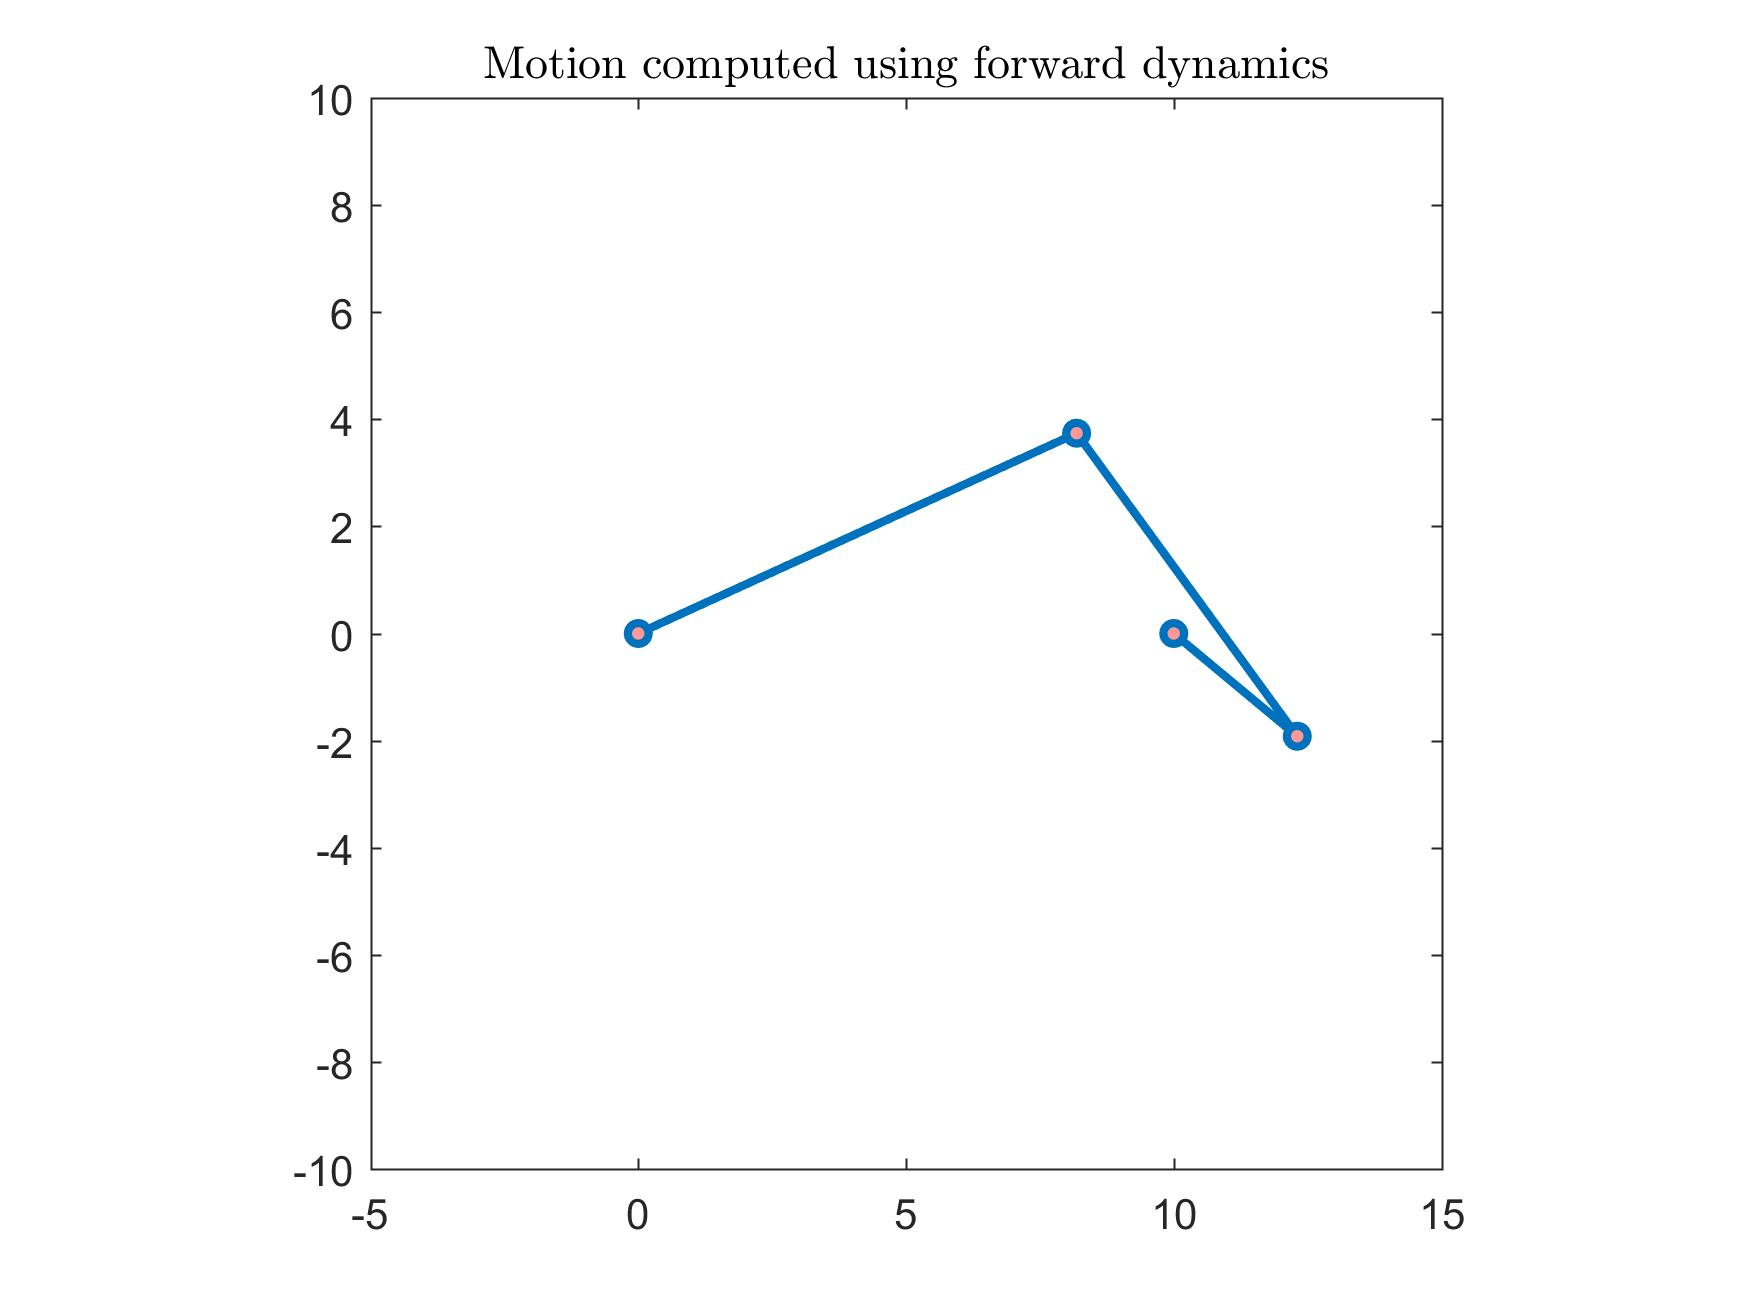
\includegraphics[width=4cm,keepaspectratio]{rockerCrank2banner}}
		\caption{\scriptsize{Rocker Crank Two}}
	\end{figure}
	\end{column}
	\begin{column}{4cm}
		\begin{table}
			\caption{\scriptsize{Parameters used for forward dynamics}}
			{\scriptsize 
				\begin{tabular}{ll}
				\hline
				$Parameter$ & $Value$ \\
				\hline
				$L_0$ & $10\; (m)$\\
				$L_1$ & $9 \; (m)$\\	
				$L_2$ & $7 \; (m)$\\
				$L_3$ & $3 \; (m)$\\
				$m_1$ & $0.5\; Kg$ \\	
				$m_2$ & $0.7\; Kg$\\
				$m_3$ & $0.6\; Kg$\\
				\hline
			\end{tabular}
		}
		\end{table}
	\end{column}
\end{columns}
\end{frame}


\begin{frame}
\frametitle{Heuristics for restarting ODE (contd...)}
\begin{columns}
	\begin{column}{4cm}
		\begin{figure}
			\centering
			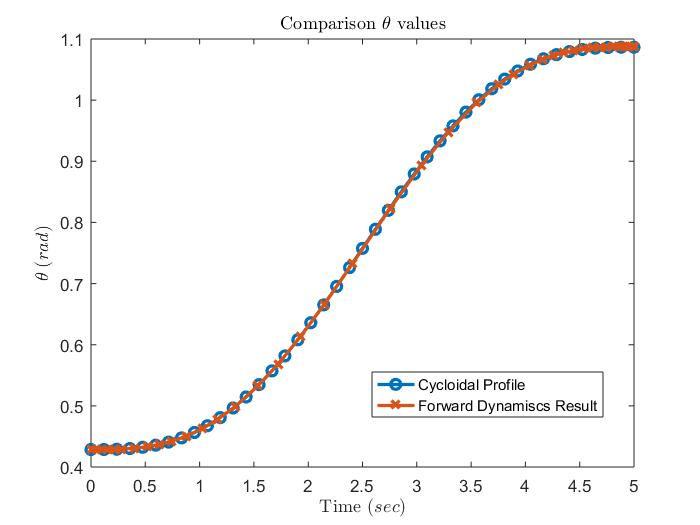
\includegraphics[width=3.5cm,keepaspectratio]{rockerCrank1position}
		\end{figure}
		\begin{figure}
			\centering
			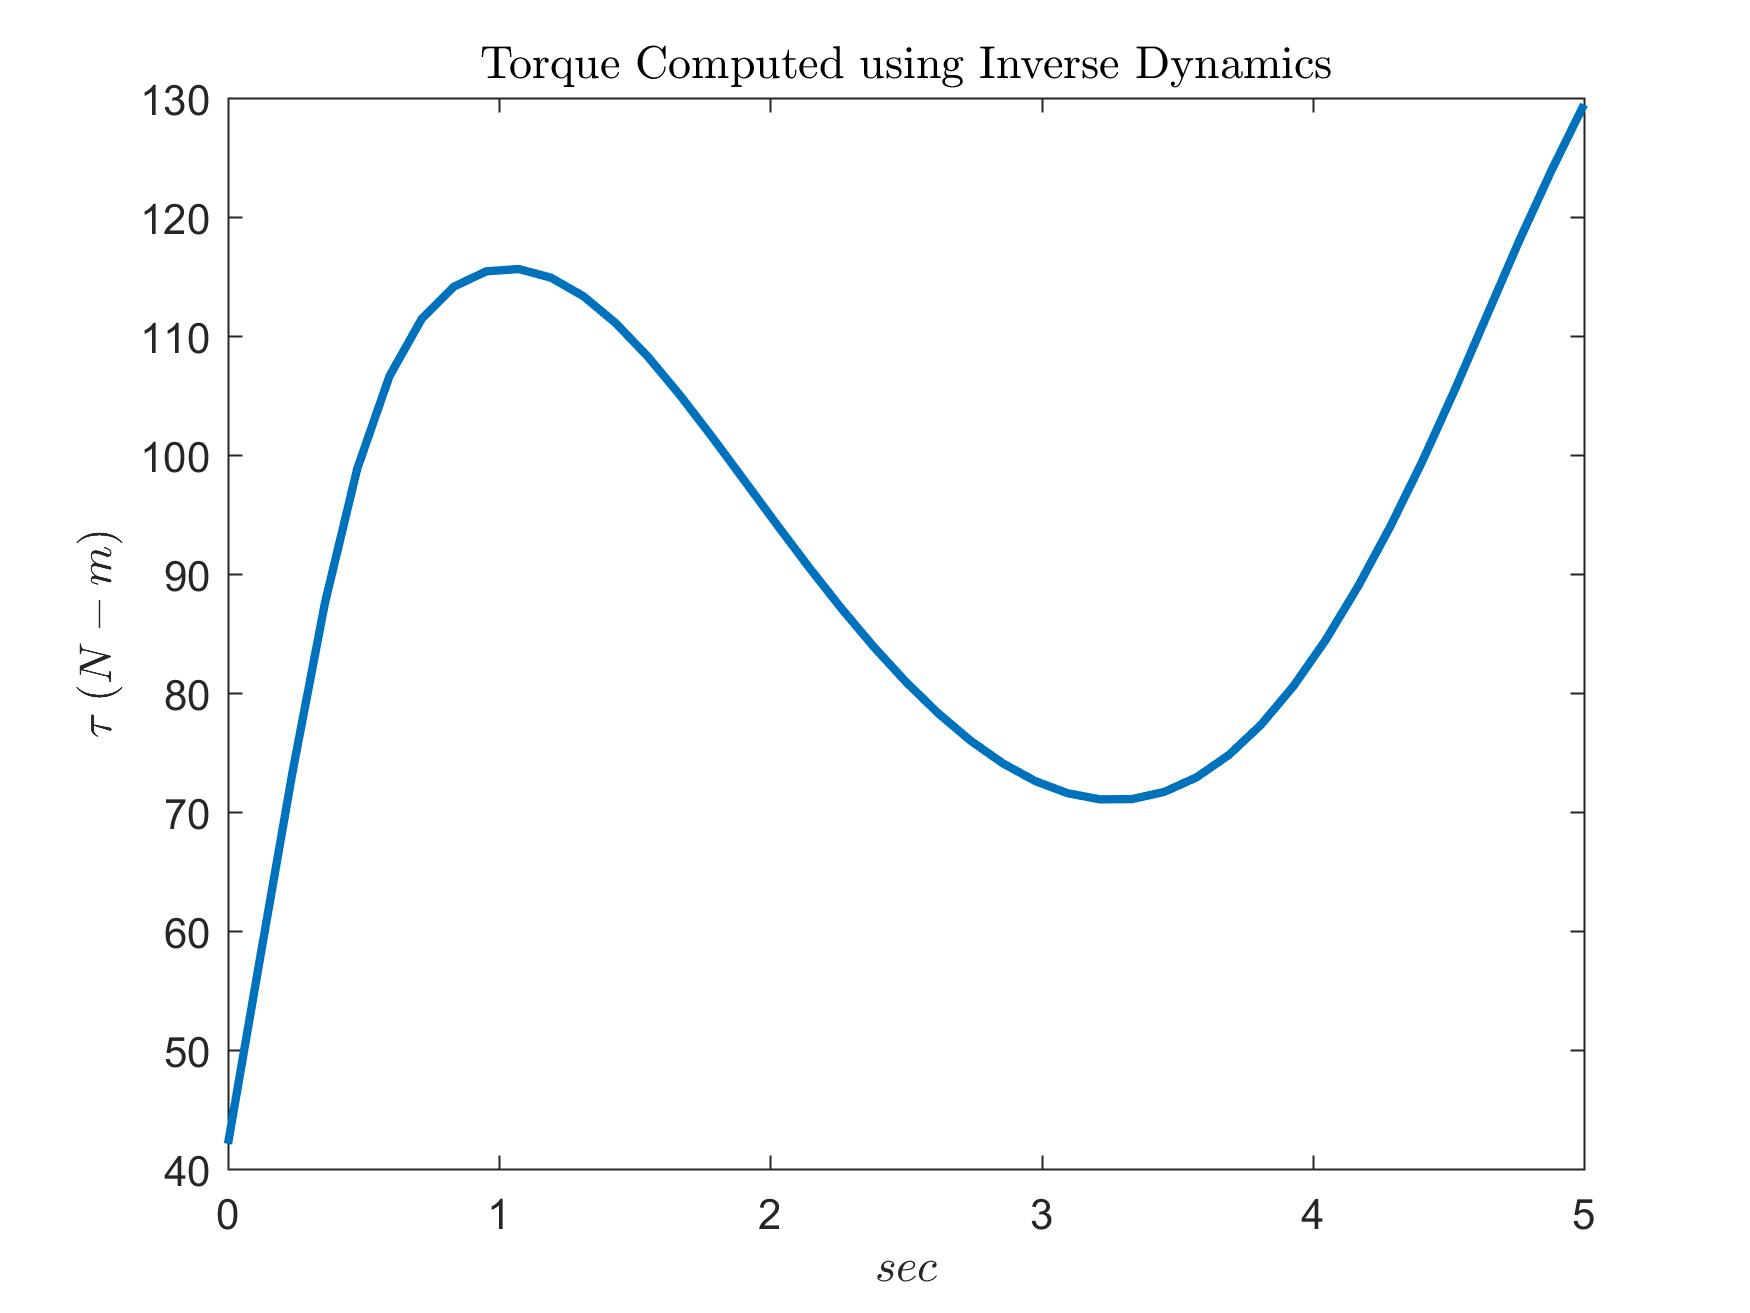
\includegraphics[width=3.5cm,keepaspectratio]{rockerCrank1TorqueInput}
	\end{figure}
	\end{column}
	\begin{column}{4cm}
		\begin{figure}
			\centering
			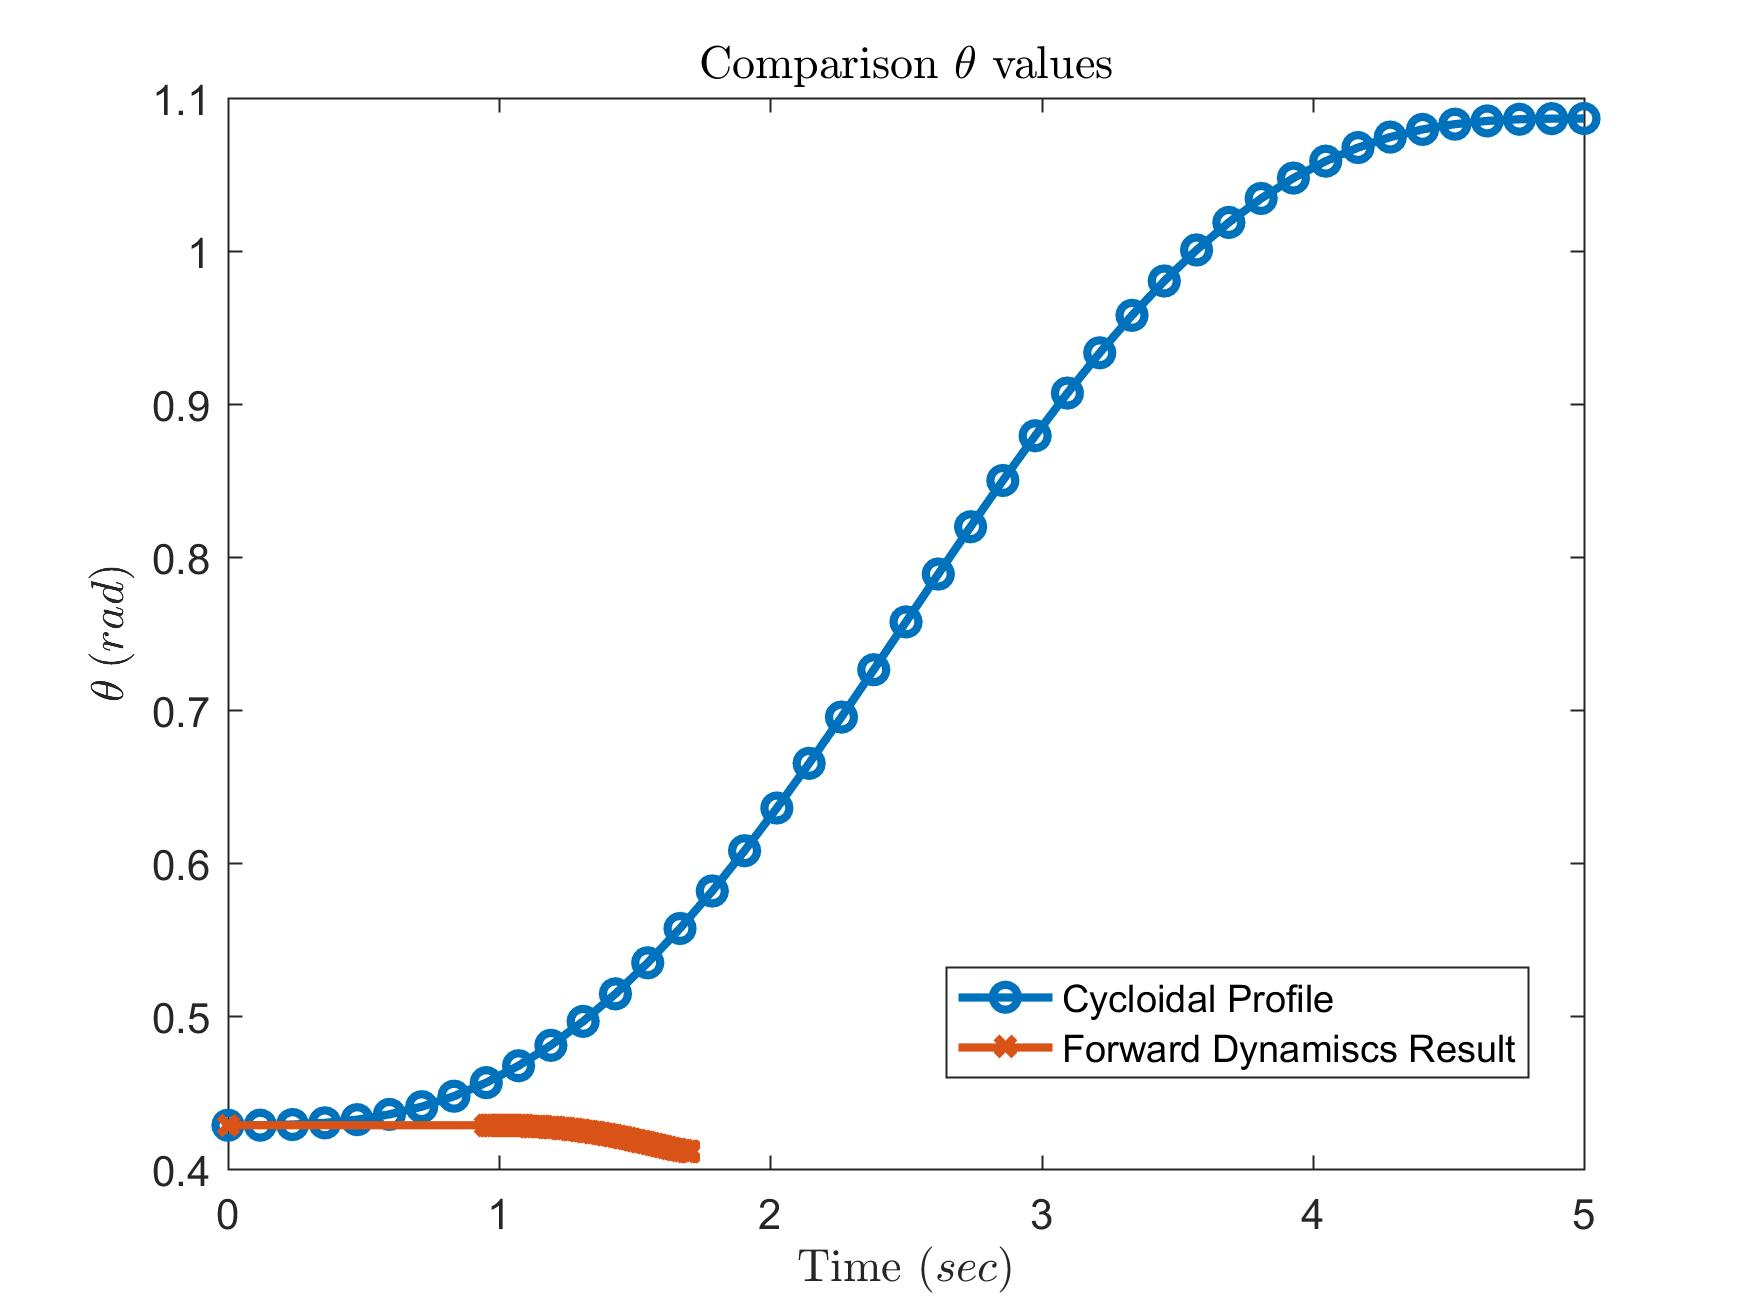
\includegraphics[width=3.5cm,keepaspectratio]{rockerCrank2position}
		\end{figure}
		\begin{figure}
			\centering
			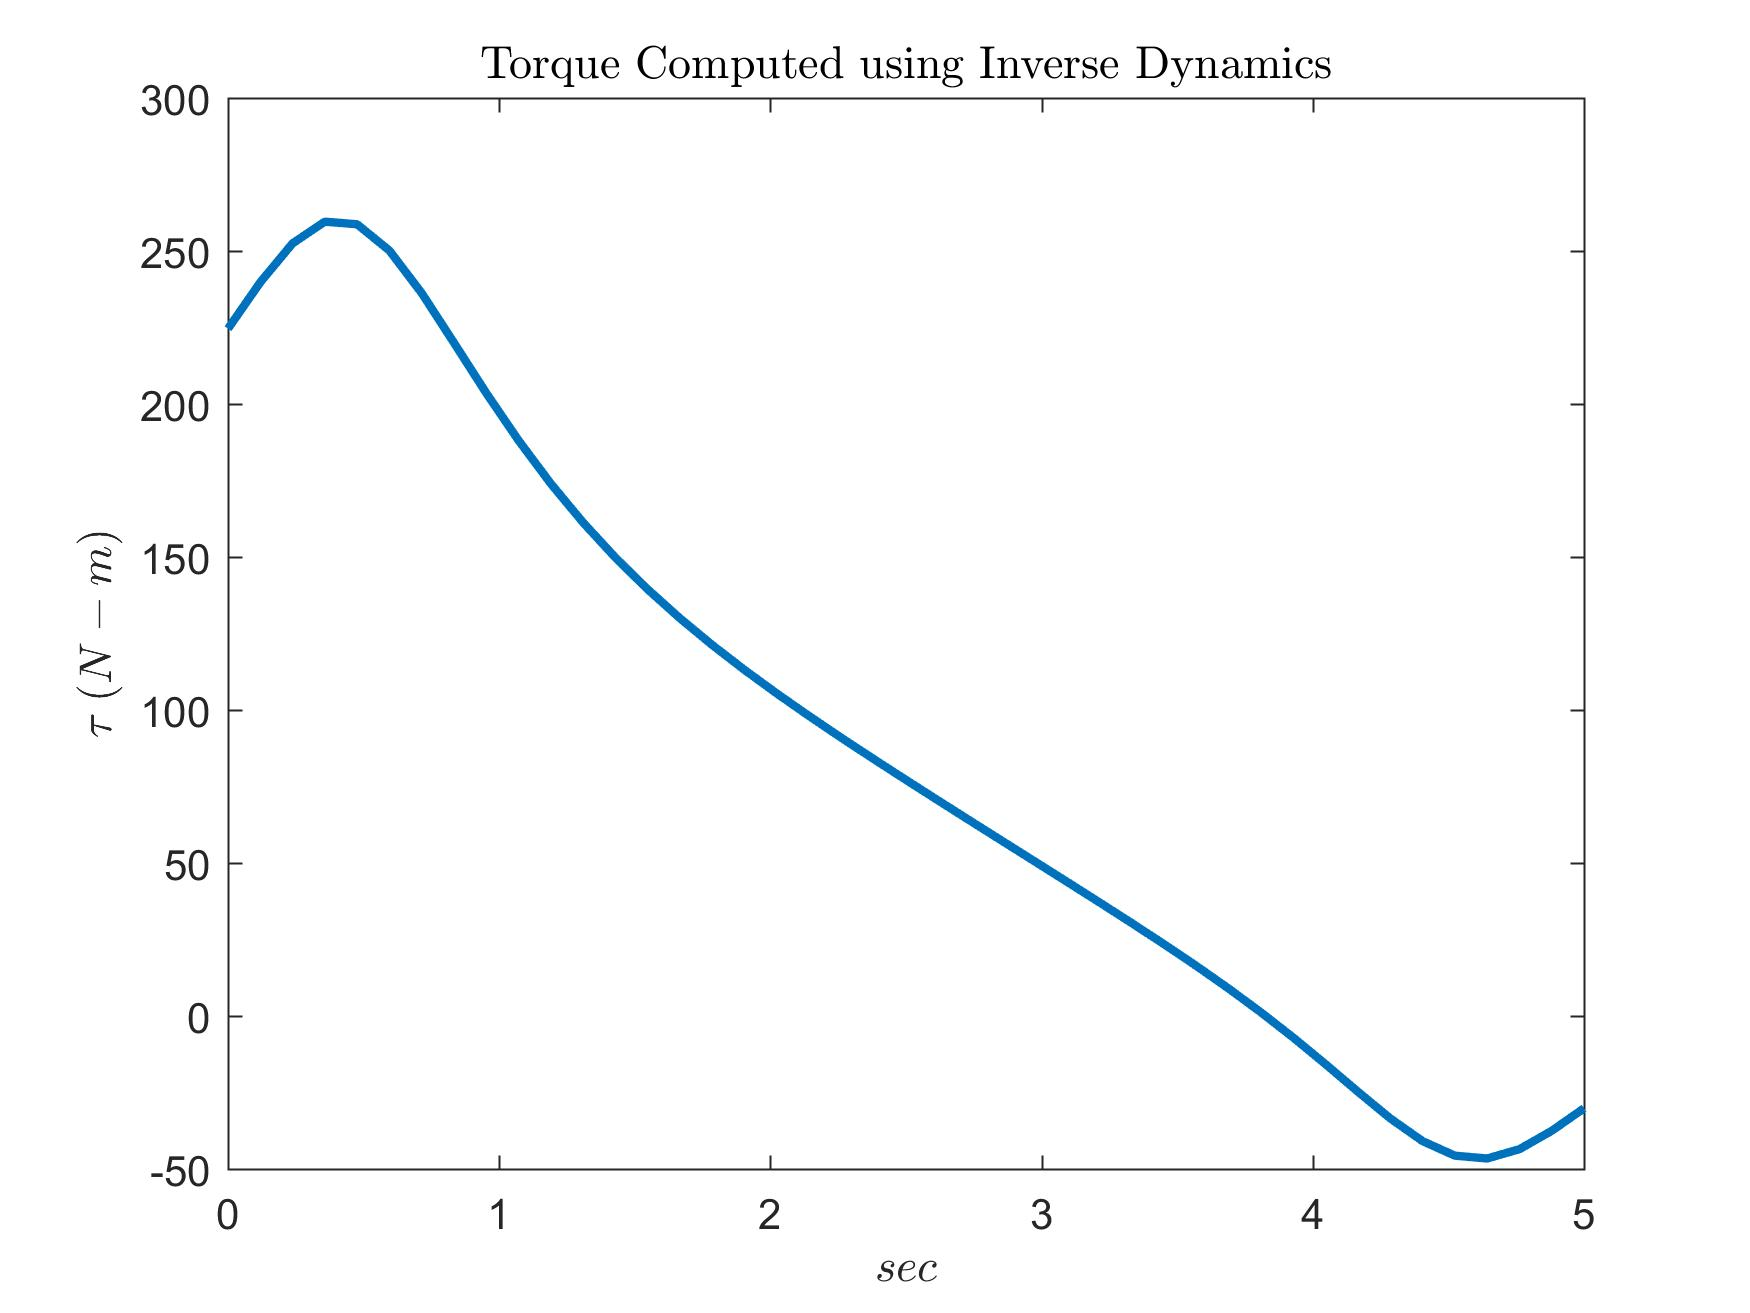
\includegraphics[width=3.5cm,keepaspectratio]{rockerCrank2TorqueInput}
		\end{figure}
	\end{column}
	\begin{column}{5cm}
		{\small In the second configuration since the input interpolated torque is small to make the link move, the ode fails to start again}
	\end{column}
\end{columns}
\end{frame}

\usebackgroundtemplate{
	\tikz[overlay,remember picture] \node[opacity=0.1, at=(current page.center)] {
		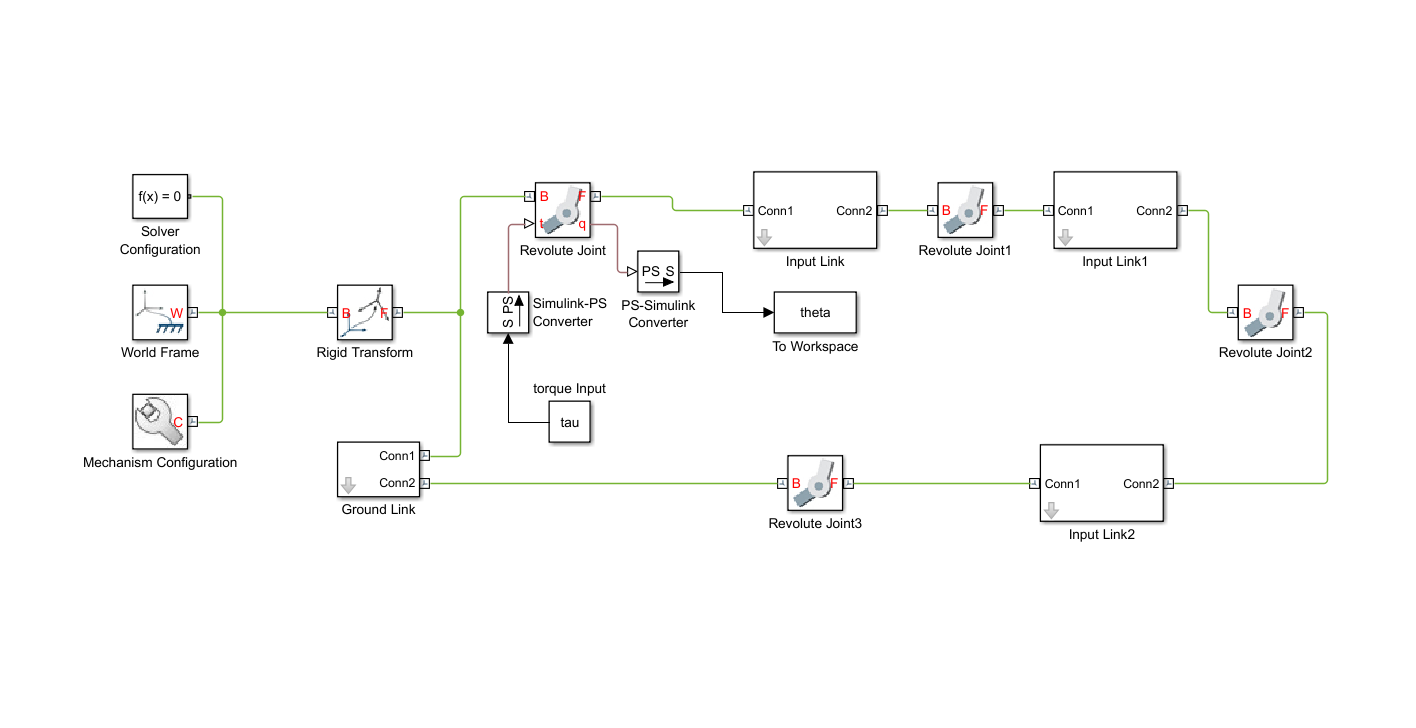
\includegraphics[height=\paperheight,width=\paperwidth]{Capture.PNG}};
}
\begin{frame}
\frametitle{The Recurdyn Alternative ????}
{\scriptsize  A constant torque of $6 \;N-m$ was applied to input link both in simMechanics and Matlab code. The close proximity of the two trajectories shows that the code was bug free.}
\begin{columns}
	\begin{column}{5cm}
		\begin{figure}
			\centering
			\href{run:./figure/theValidationVideo.avi}{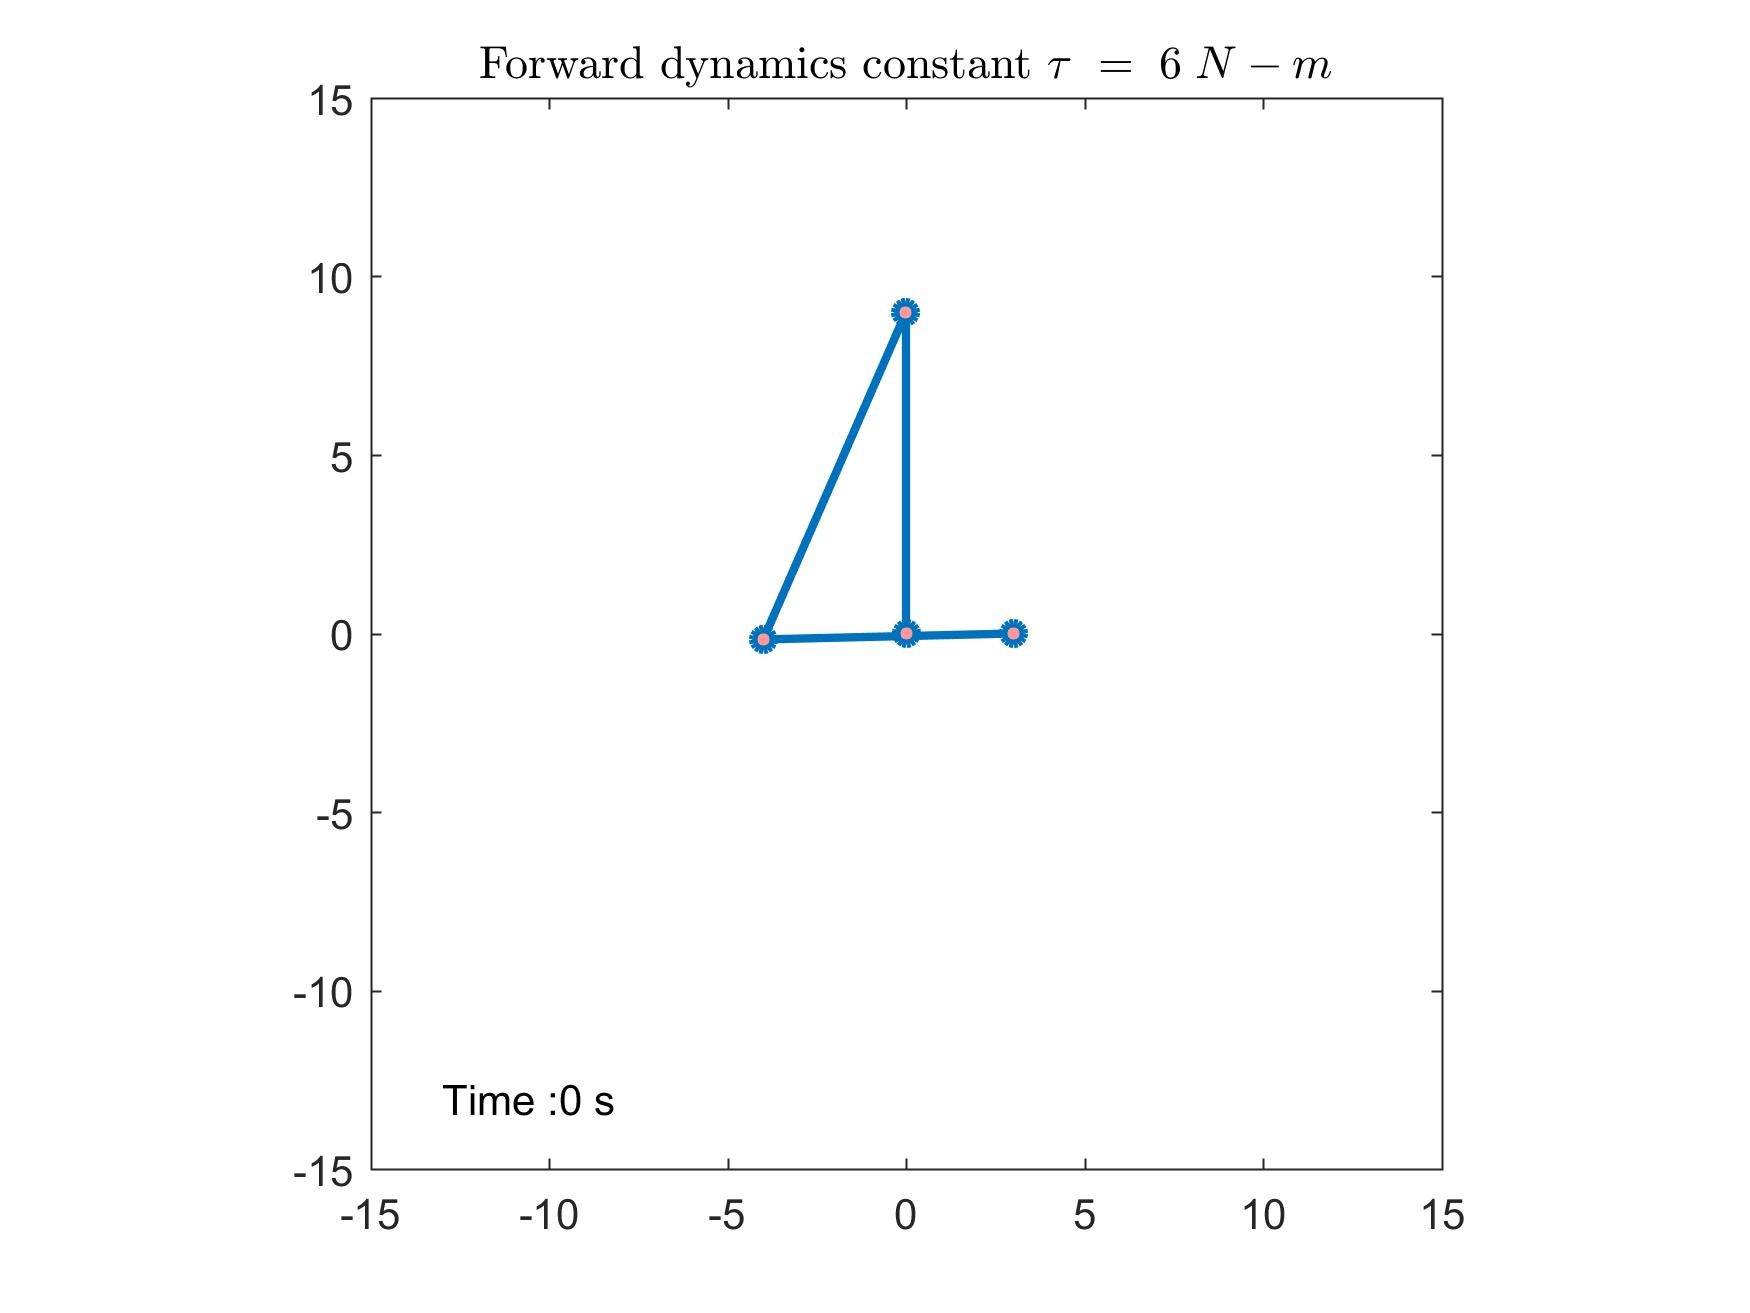
\includegraphics[width=3.7cm,keepaspectratio]{theValidationBanner}}
		\end{figure}
		\begin{figure}
			\centering
			\href{run:./figure/fourbarSimMechanics.avi}{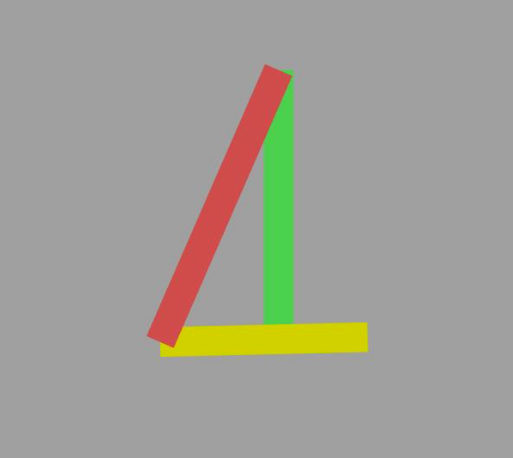
\includegraphics[width=2.5cm,keepaspectratio]{fourbarSimMechanicsBanner}}
		\end{figure}
	\end{column}
	\begin{column}{6cm}
		\begin{figure}
			\centering
			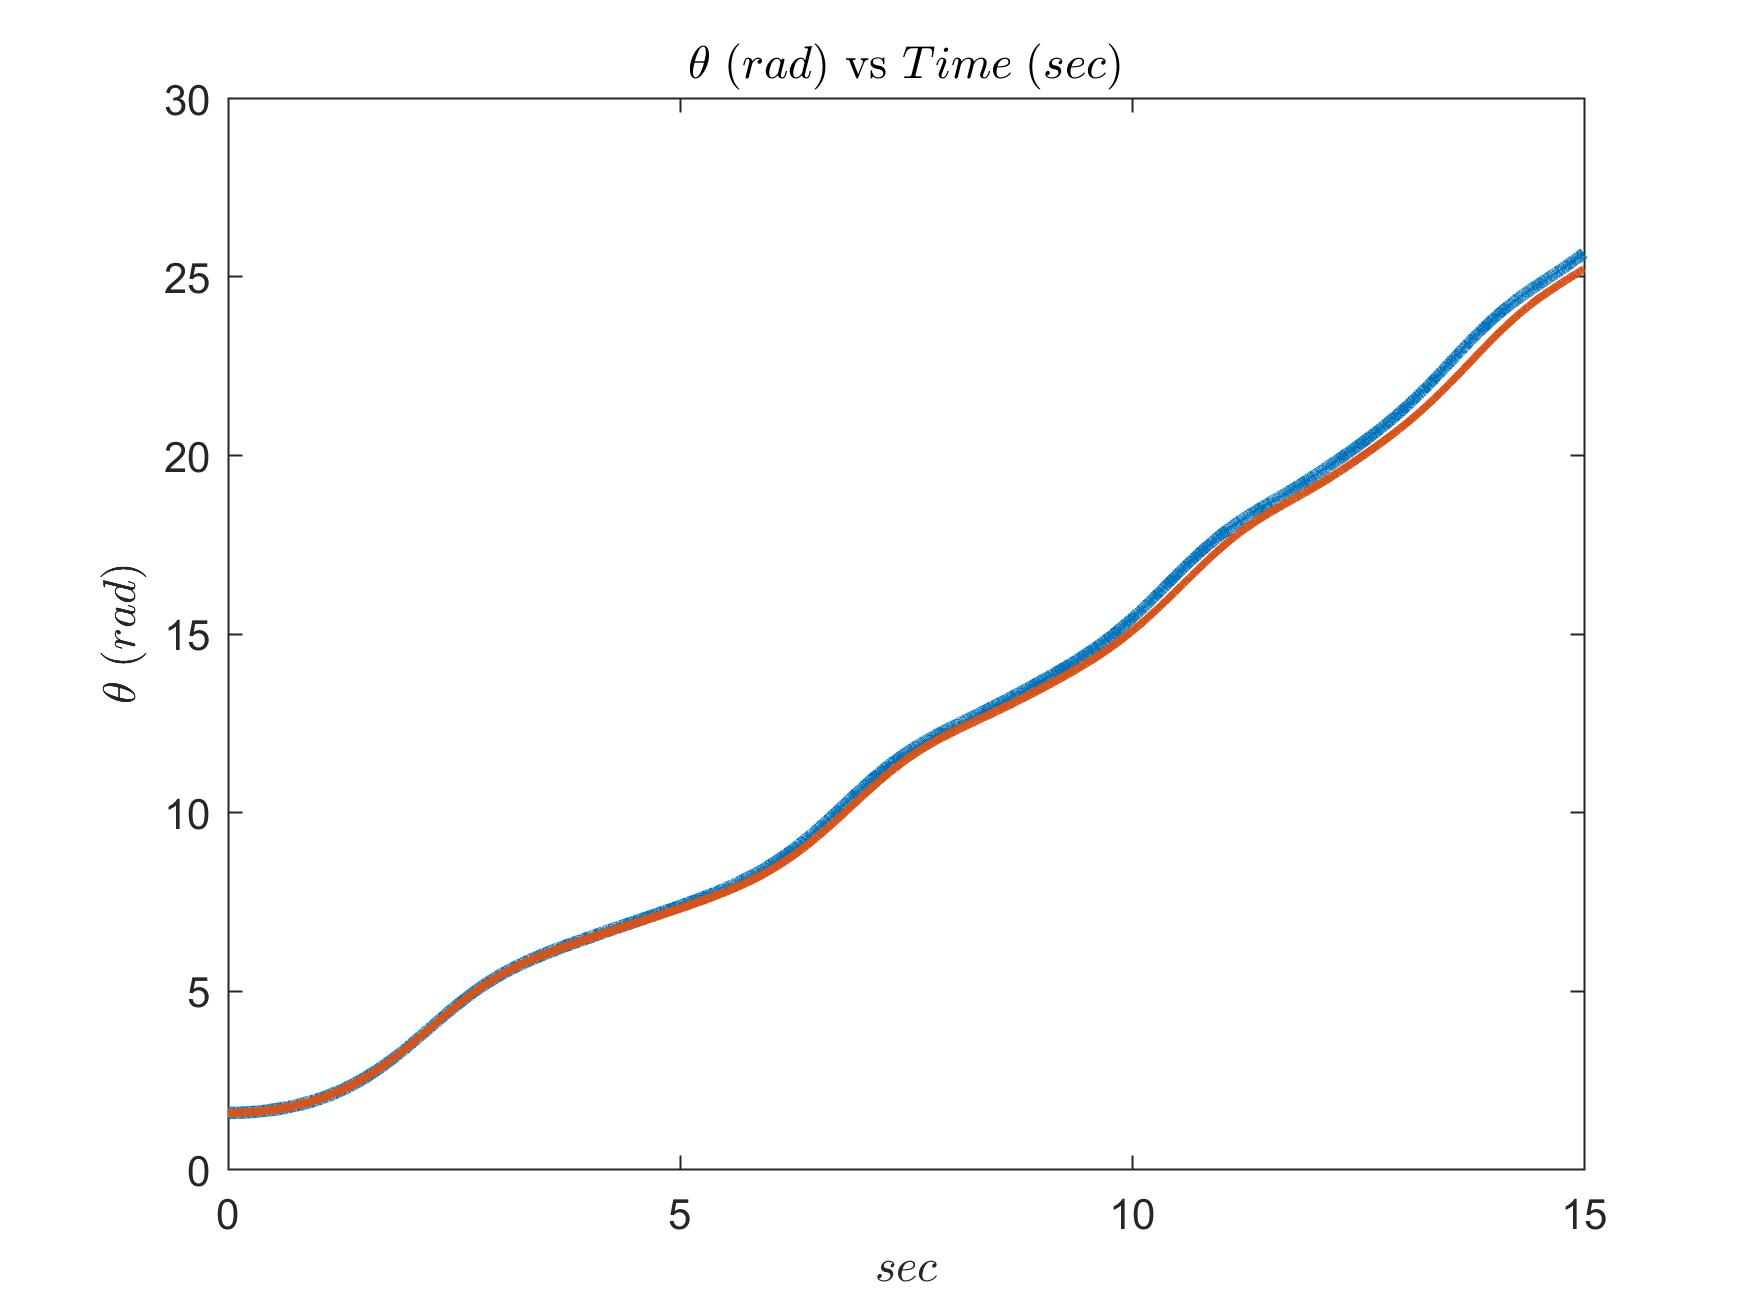
\includegraphics[width=6cm,keepaspectratio]{theValidation}
			\caption{$\theta \; vs \; time$}
		\end{figure}
	\end{column}
	
	\begin{column}{4cm}
	\begin{table}
		\caption{Parameters used for forward dynamics}
		{\scriptsize 
			\begin{tabular}{ll}
				\hline
				$Parameter$ & $Value$ \\
				\hline
				$L_0$ & $3\; m$\\
				$L_1$ & $9\; m$ \\	
				$L_2$ & $10\; m$\\
				$L_3$ & $7\; m$\\
				$m_1$ & $1\; Kg$ \\	
				$m_2$ & $1\; Kg$\\
				$m_3$ & $1\; Kg$\\
				$\theta$ & $\pi/2\; (rad)$\\
				$\dot{\theta}$ & $0\; (rad/sec)$\\
				$\tau$ & $6\; N-m$\\
				\hline
			\end{tabular}
		}
	\end{table}
	\end{column}
\end{columns}
\end{frame}
\usebackgroundtemplate{ }

\begin{frame}
\frametitle{Its All About "Energy"}
{\scriptsize A constant torque of $6\; N-m$ applied to the input link, for same link lengths as that of previous slides but with second mode of assembly.}
\begin{columns}
	\begin{column}{6cm}
		\begin{figure}
			\centering
			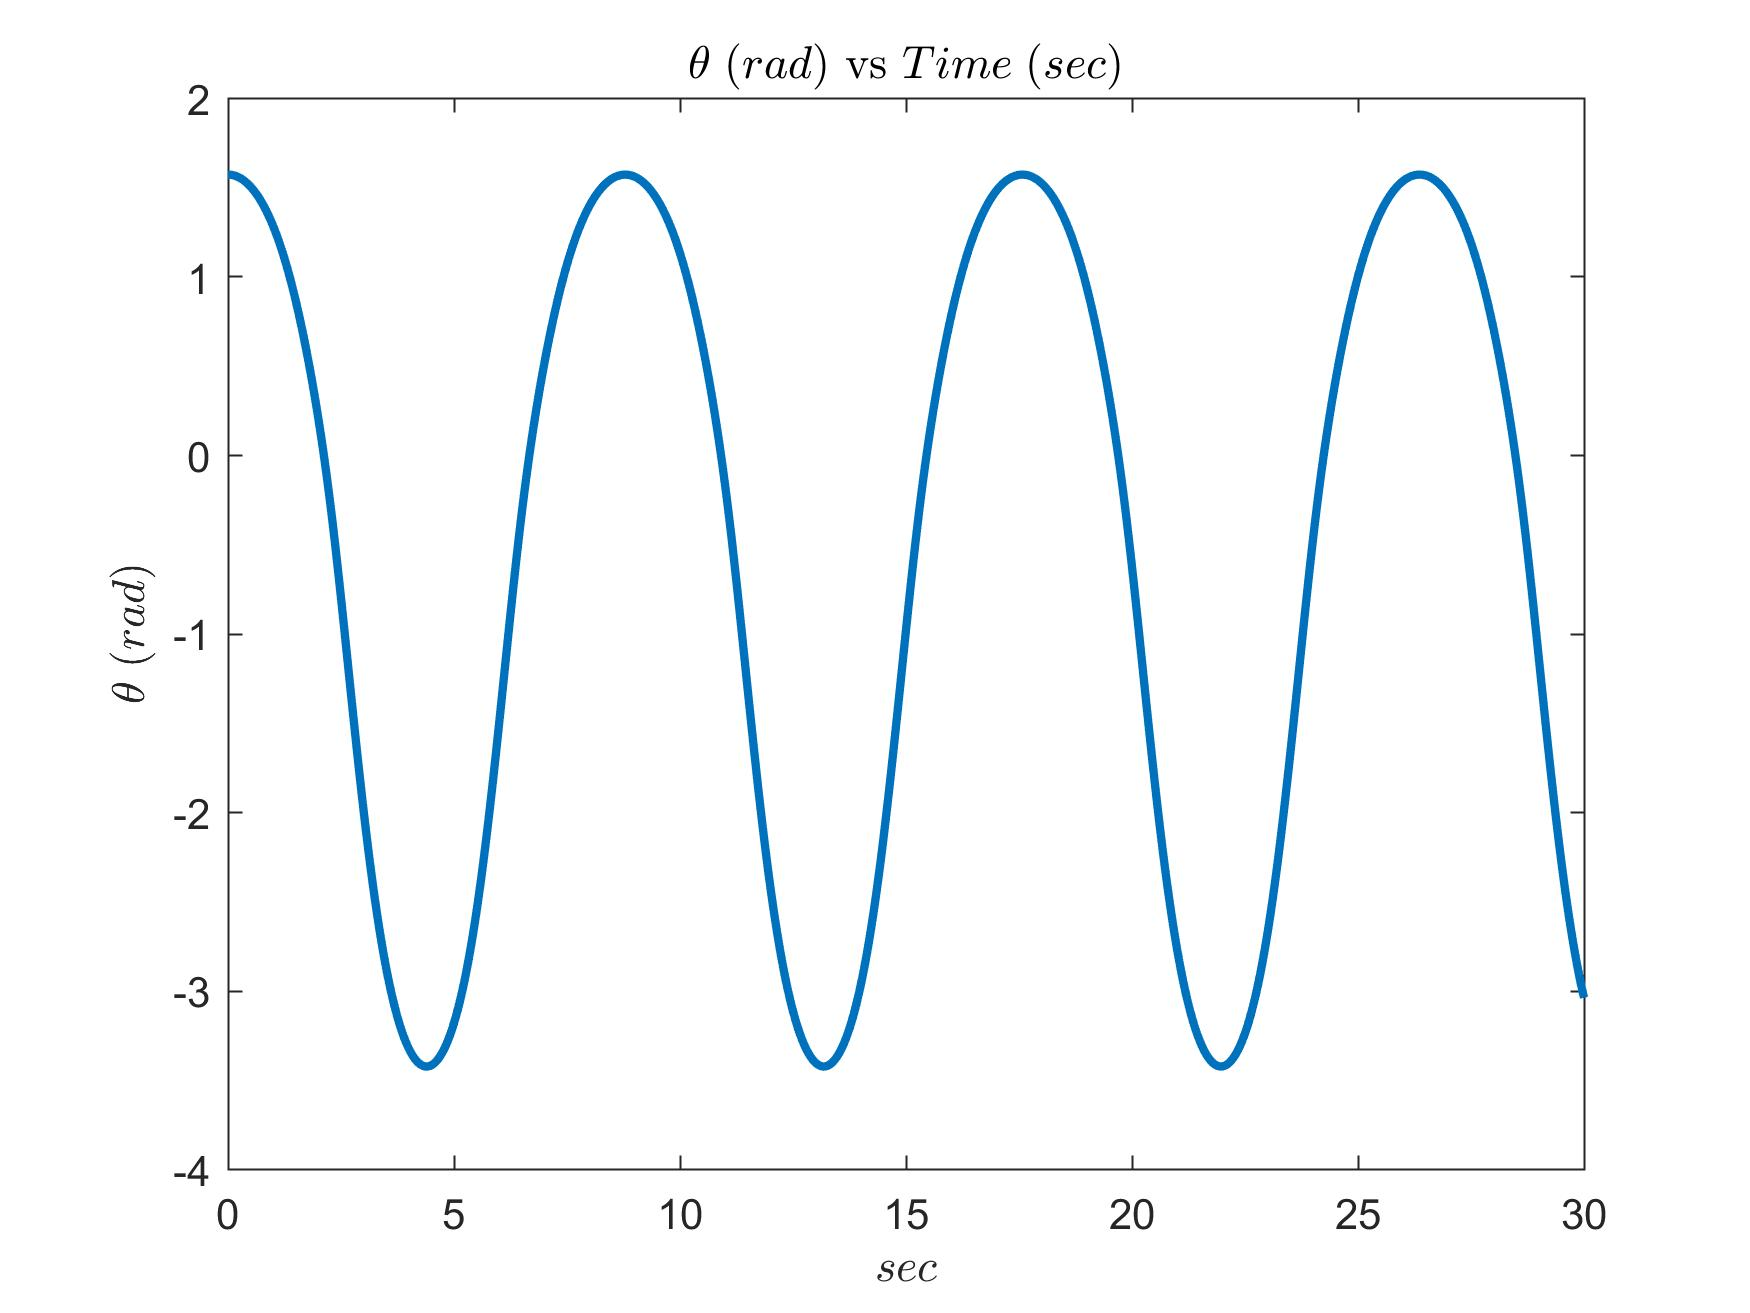
\includegraphics[width=6cm,keepaspectratio]{fourBarPendulum}
			\caption{$\theta \; vs \; time$}
		\end{figure}
	\end{column}
	\begin{column}{6cm}
		\begin{figure}
			\centering
			\href{run:./figure/fourBarPendulum.avi}{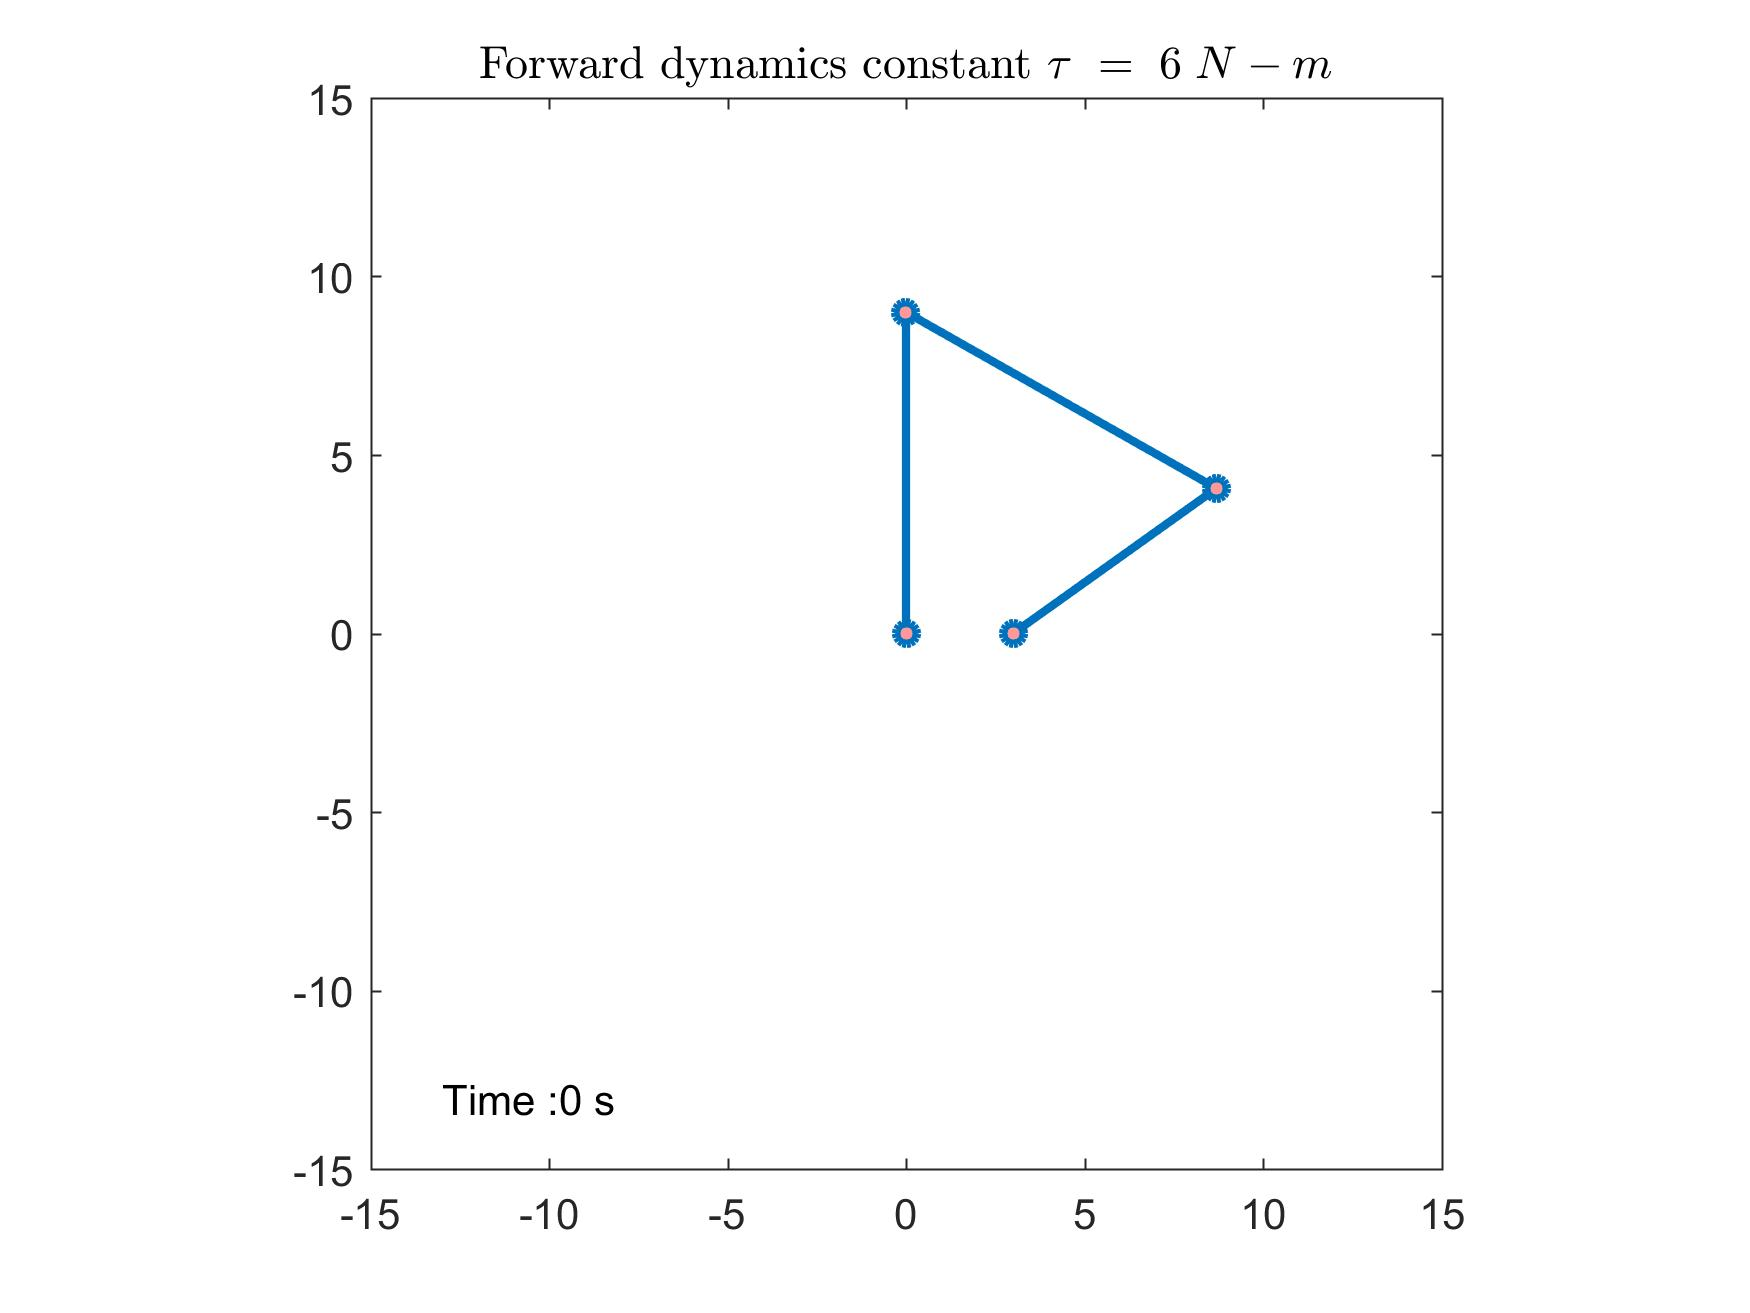
\includegraphics[width=6cm,keepaspectratio]{fourBarPendulumBanner}}
		\end{figure}
	\end{column}
\end{columns}
\end{frame}

\begin{frame}
\frametitle{Some Pretty Videos}
\begin{columns}	
	\begin{column}{3cm}
		\centering
		\href{run:./figure/crankCrank1Forward.avi}{\beamergotobutton{Crank Crank One}}	\\
		\href{run:./figure/crankRocker1Forward.avi}{\beamergotobutton{Crank Rocker One}}	\\
		\href{run:./figure/rockerCrank1Forward.avi}{\beamergotobutton{Rocker Crank One}}	\\
		\href{run:./figure/rockerRocker1Forward.avi}{\beamergotobutton{Rocker Rocker One}}
	\end{column}
	\begin{column}{3cm}
		\centering
		\href{run:./figure/crankCrank2Forward.avi}{\beamergotobutton{Crank Crank Two}}	\\
		\href{run:./figure/crankRocker2Froward.avi}{\beamergotobutton{Crank Rocker Two}}	\\
		\href{run:./figure/rockerCrank2Forward.avi}{\beamergotobutton{Rocker Crank Two}}	\\
		\href{run:./figure/rockerRocker2Forward.avi}{\beamergotobutton{Rocker Rocker Two}}
	\end{column}
	\begin{column}{3cm}
		\begin{table}
			{\scriptsize 
				\begin{tabular}{ll}
					\hline
					$Parameter$ & $Value$ \\
					\hline
					$L_0$ & $10\; (m)$\\
					$L_1$ & $9 \; (m)$\\	
					$L_2$ & $7 \; (m)$\\
					$L_3$ & $3 \; (m)$\\
					$m_1$ & $0.5\; Kg$ \\	
					$m_2$ & $0.7\; Kg$\\
					$m_3$ & $0.6\; Kg$\\
					\hline
				\end{tabular}
			}
		\end{table}
	\end{column}
\end{columns}

\end{frame}


\begin{frame}
\frametitle{References}
\bibliographystyle{ieeetr}
{\footnotesize \bibliography{references}}
\end{frame}

\begin{frame}
\centering
\frametitle{.}
\LARGE{Thank You}\\
	
\end{frame}

\end{document}